\chapter{Analyse et Conception}
\vspace{5cm}
\large{Ce deuxième chapitre présente tout d’abord d’une manière générale La méthode que nous avons adopté pour réaliser l'analyse et la conception de notre système d'information.\\}


\newpage
\section{Méthode adoptée}
\large{La méthode que nous avons adopté pour réaliser l'analyse et la conception de notre système d'information est la méthode UML : Elle permet la séparation entre les données et les traitements effectués en plusieurs modèles conceptuels qui sont répartis sur 3 diagrammes : Le diagramme de cas d'utilisation, le diagramme de classe,diagramme de séquence. Dans cette partie, nous allons présenter quelques-unes de ces méthodes, et en denissant par les maquettes. Cette phase a pour objectif de déduire la spécication de l'architecture du système.\\}
\section{Diagramme de cas d'utilisations}
\large{les diagrammes de cas d'utilisation modélisent le comportement d'un système et permettent de capturer les exigences du système. Les diagrammes de cas d'utilisation décrivent les fonctions générales et la portée d'un système. Ces diagrammes identident également les interactions entre le système et ses acteurs. Les cas d'utilisation et les acteurs dans les diagrammes de cas d'utilisation décrivent ce que le système fait et comment les acteurs l'utilisent, mais ne montrent pas comment le système fonctionne en interne.}

%\subsection{Admin}
%\begin{page}{\textwidth}
%	\begin{page}{\linewidth}
%	\makebox[\linewidth]{
%		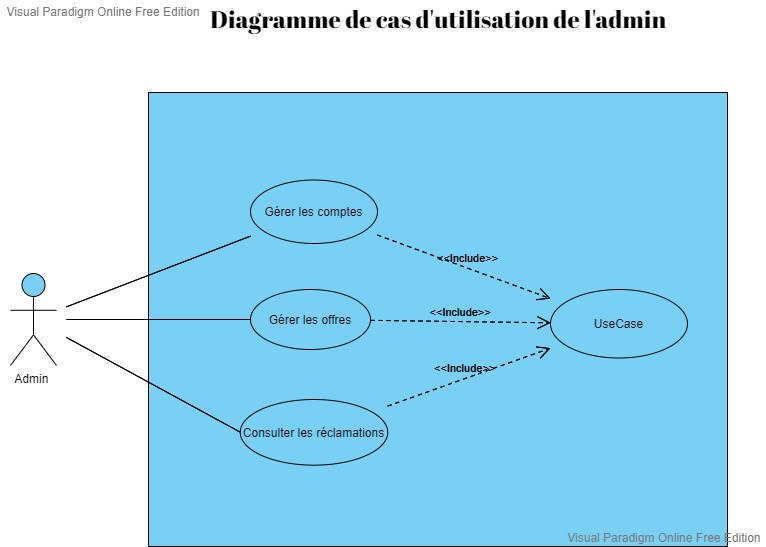
\includegraphics[keepaspectratio=true,scale=0.38]{uc1.jpeg}} 
%		\captionof{figure}{Diagramme de cas d'utilisation admin}\label{f3}%
%\end{page}
%\end{page}

\subsection{Utilisateur/visiteur}

\begin{page}{\textwidth}
	\begin{page}{\linewidth}
	\makebox[\linewidth]{
		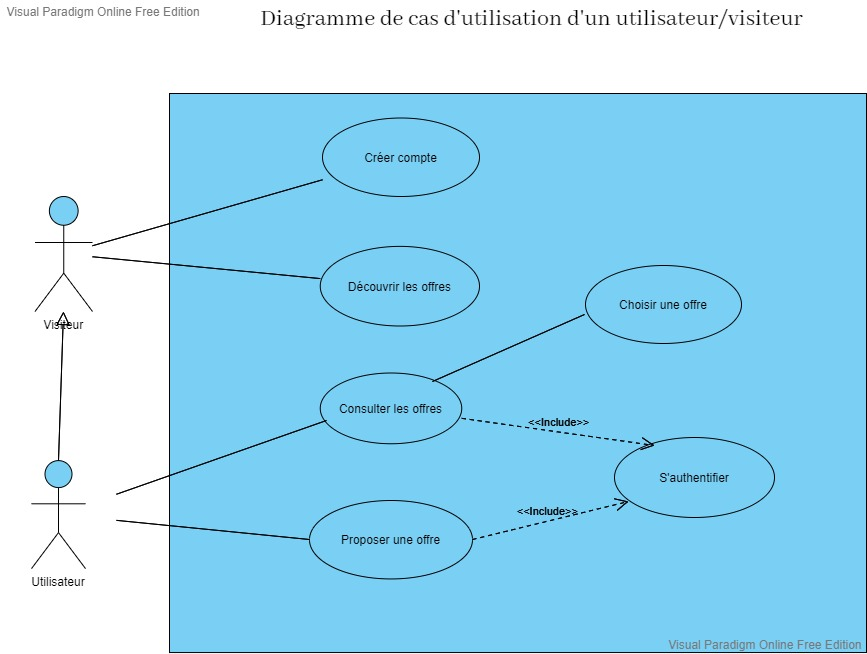
\includegraphics[keepaspectratio=true,scale=0.38]{uc2.jpeg}} 
		\captionof{figure}{Diagramme de cas d'utilisation utilisateur/visiteur}\label{f3}%
\end{page}
\end{page}
\newpage
\section{Diagramme de classe}
\begin{page}{\textwidth}
	\begin{page}{\linewidth}
	\makebox[\linewidth]{
		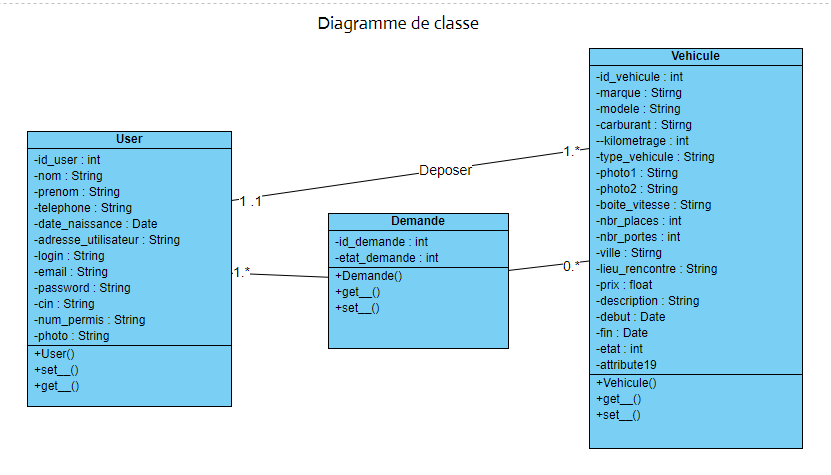
\includegraphics[keepaspectratio=true,scale=0.9]{diagramme_de_classe.png}} 
		\captionof{figure}{Diagramme de classe}\label{f3}%
\end{page}
\end{page}
\newpage

\section{Diagramme de séquences}
\large{Pour schématiser la vue comportementale de notre système informatique, nous faisons recours au diagramme
de séquence d'UML. Ce diagramme permet de présenter les interactions entre l'acteur et le système avec des
messages présentés dans un ordre chronologique. Le diagramme de séquences traite le système informatique
comme étant une boite noire. Le comportement du système est décrit de l'extérieur sans avoir d'idée sur la
réalisation. Nous pouvons, alors, constater que certains cas d'utilisation sont similaires, c'est pourquoi nous
avons choisi de traiter quelques exemples.\\}

\newpage
\begin{figure}[p]

\centering
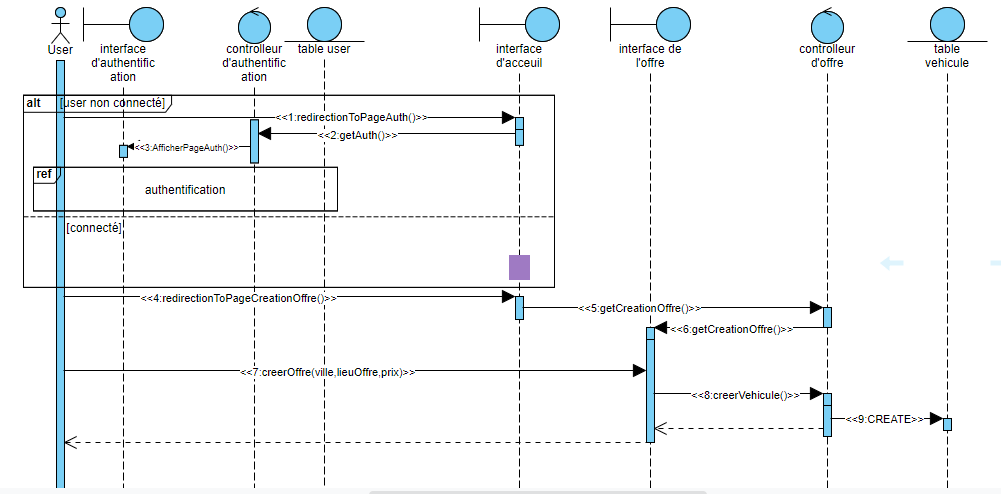
\includegraphics[width=1.3\textwidth, angle =90 ]{55.PNG}
\caption{Diagramme de séquence proposer une offre}
\label{fig:awesome_image}

\end{figure}
\newpage
\begin{figure}[p]

\centering
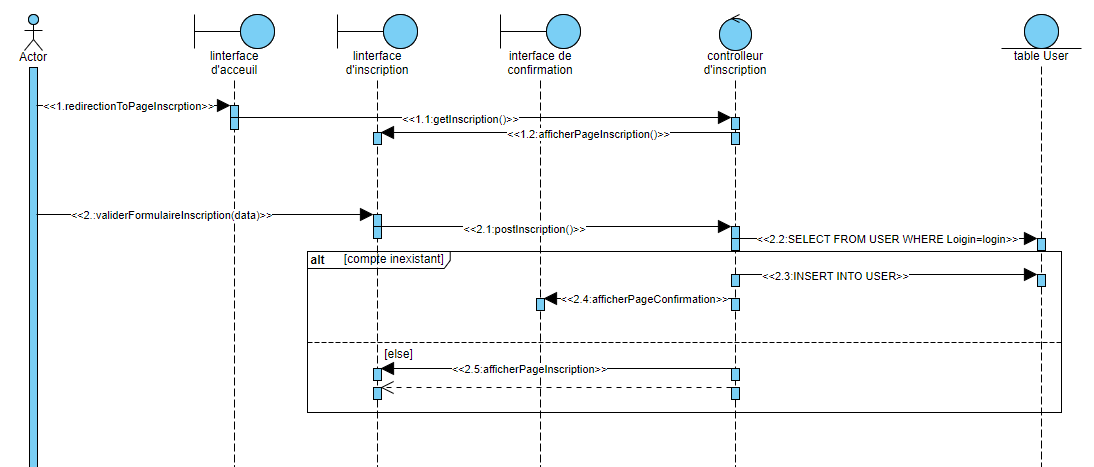
\includegraphics[width=1.3\textwidth, angle =90 ]{44.PNG}
\caption{Diagramme de séquence céer compte}
\label{fig:awesome_image}

\end{figure}
\newpage
\begin{figure}[p]

\centering
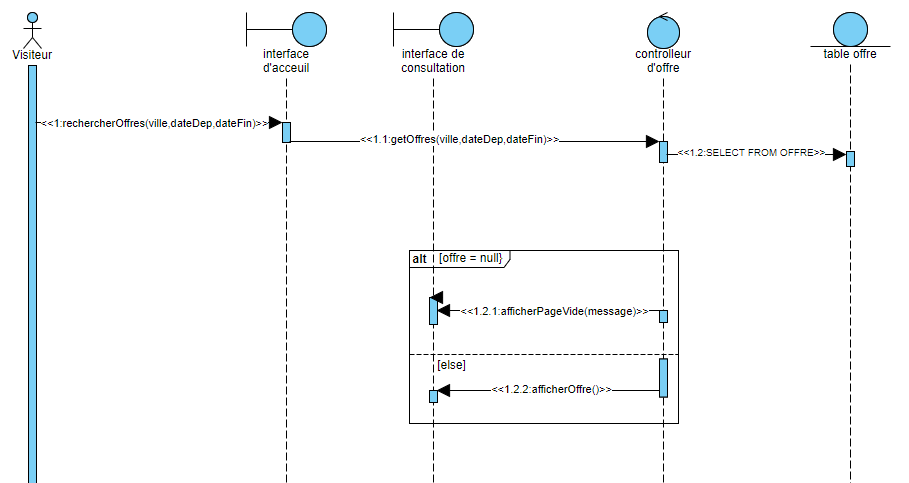
\includegraphics[width=1.3\textwidth, angle =90 ]{33.PNG}
\caption{Diagramme de séquence consulter les offres}
\label{fig:awesome_image}

\end{figure}
\newpage
\begin{figure}[p]

\centering
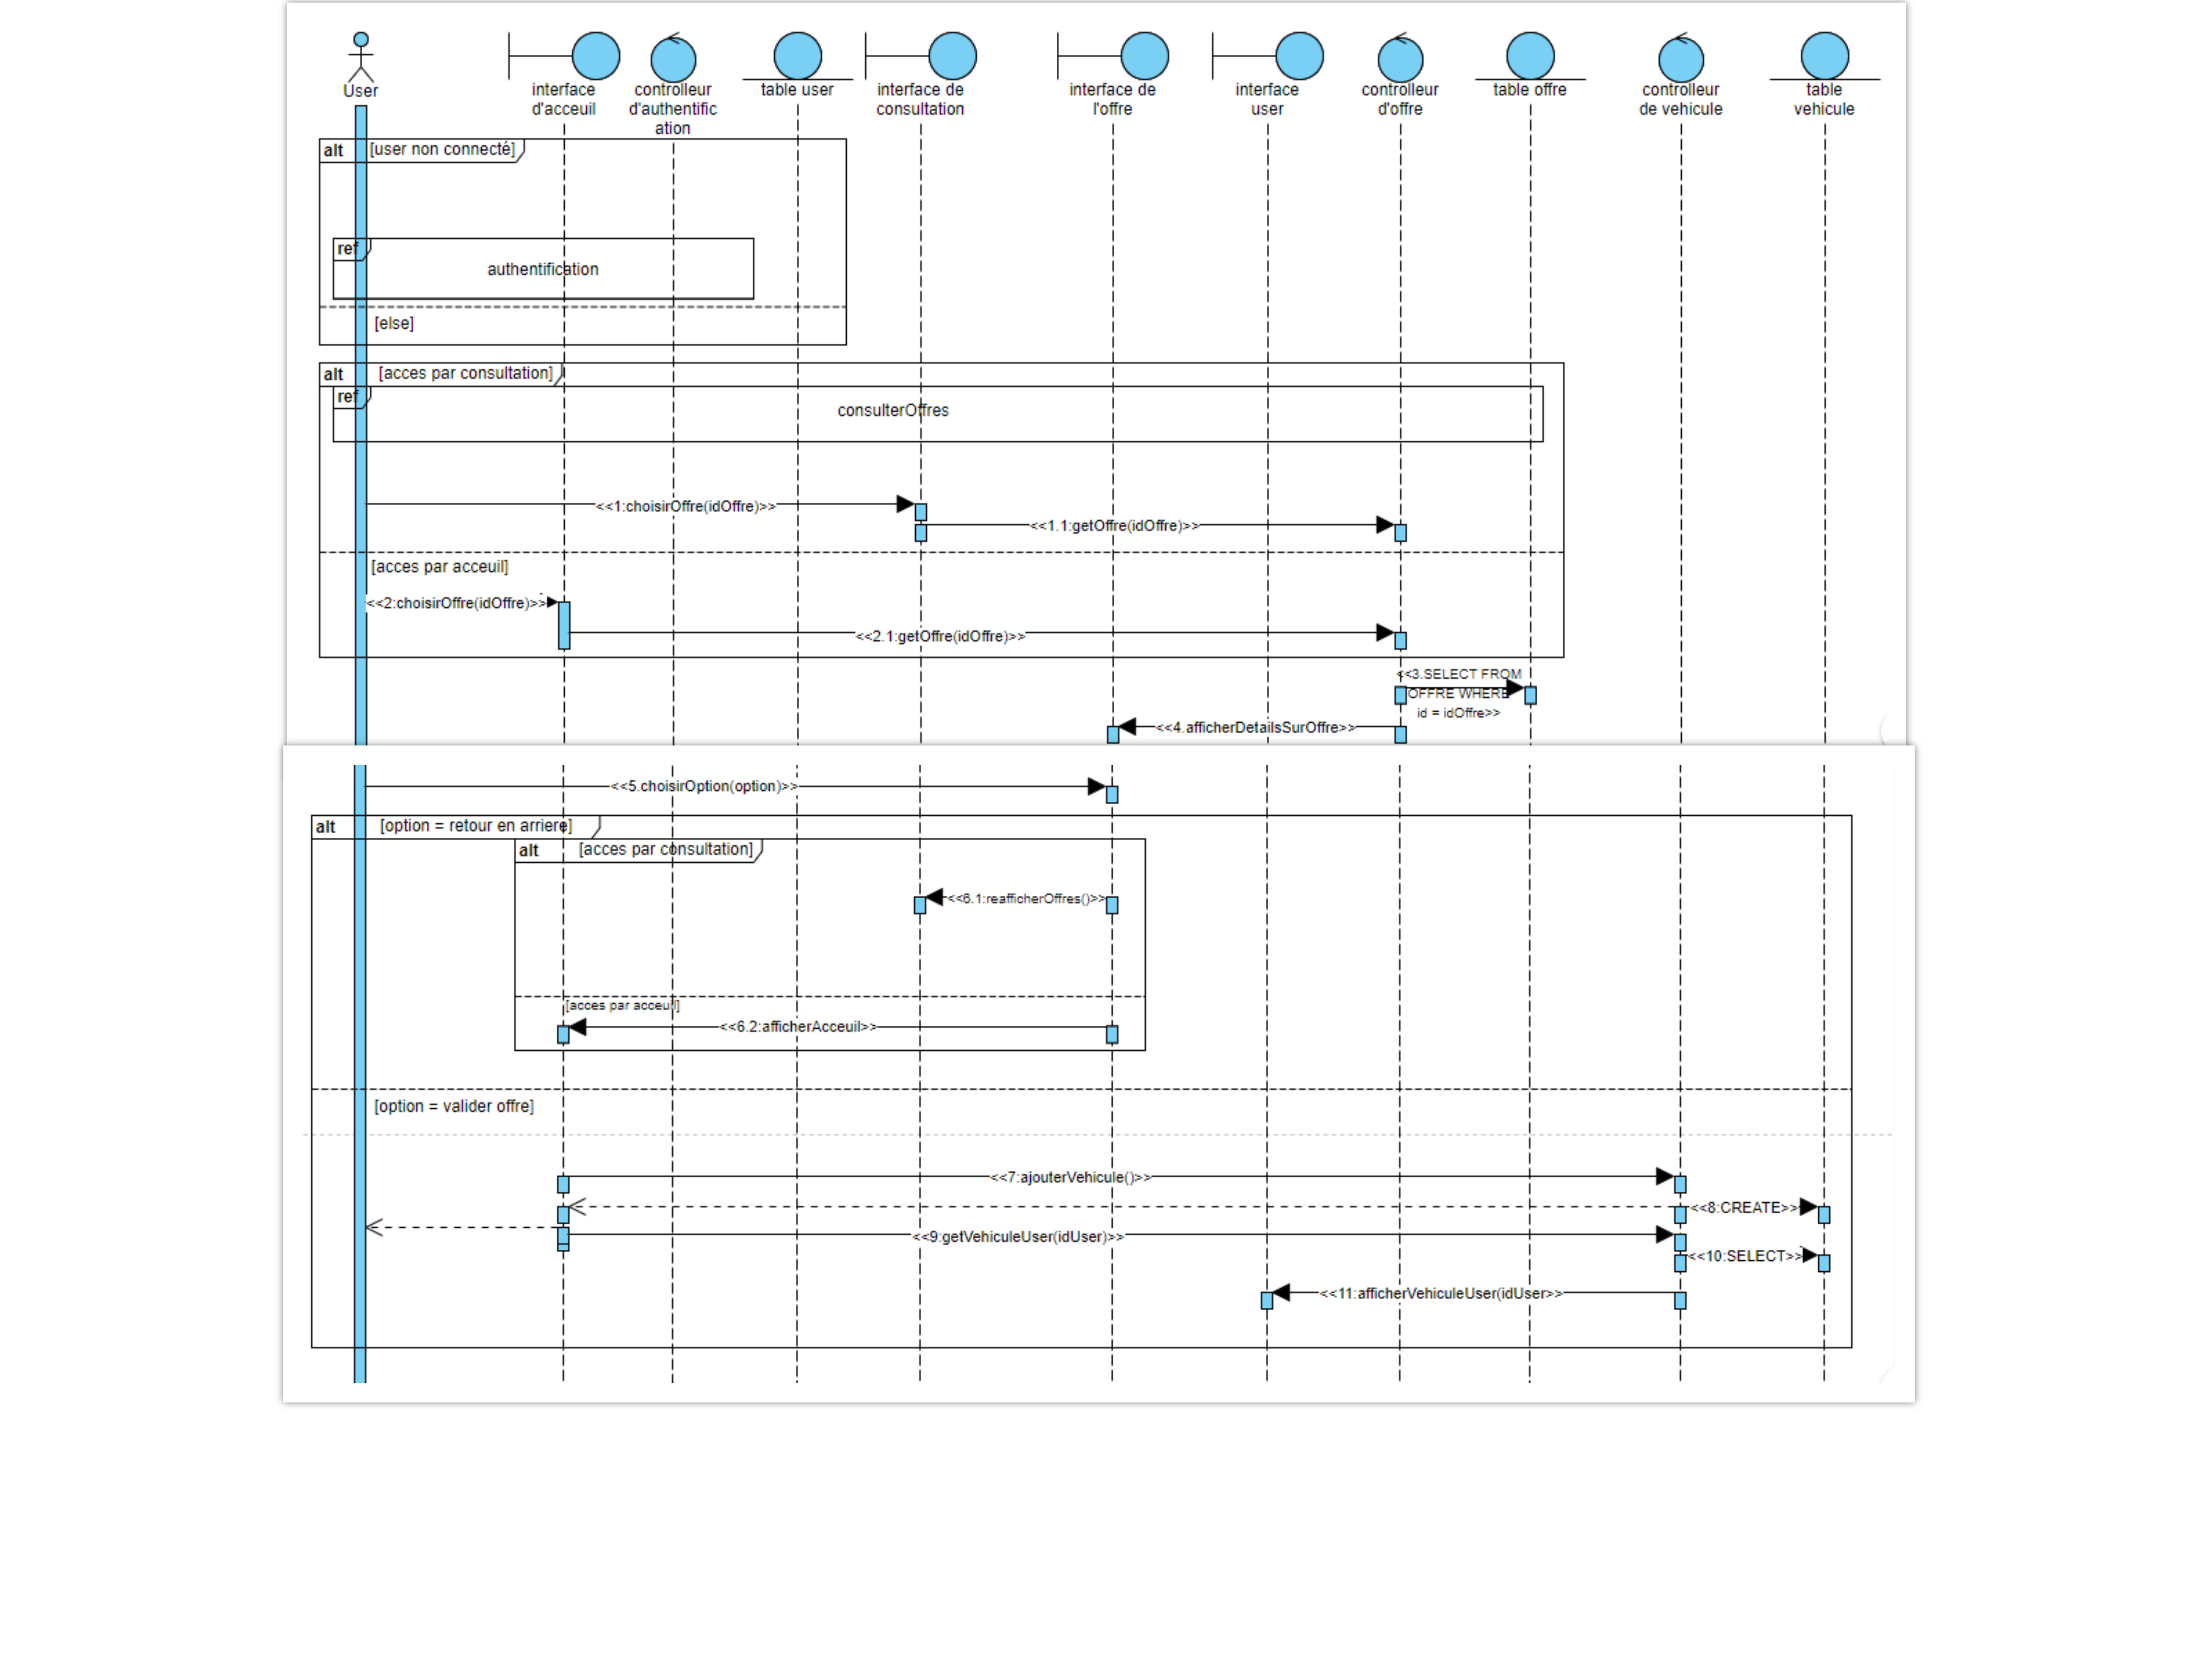
\includegraphics[width=1.3\textwidth, angle =90 ]{111.png}
\caption{Diagramme de séquence Choisir offre}
\label{fig:awesome_image}

\end{figure}
\newpage





